\documentclass[conference]{IEEEtran}
\usepackage{graphicx}
\usepackage{amsmath}

\graphicspath{{./gambar/}}

\title{Analisis kekuatan Sinyal Menggunakan inSSIDer}

\author{Kevin Antony K\IEEEauthorrefmark{1}, Maranti Nainggolan\IEEEauthorrefmark{2}\\
\textit{Fakultas Teknologi Informasi}\\
\textit{Teknik Komputer}\\
\textit{Institut Teknologi Batam}\\
Batam, Indonesia\\
Email: \{\IEEEauthorrefmark{1}1922003, \IEEEauthorrefmark{2}1922023\}@student.iteba.ac.id}

\begin{document}
\maketitle

\begin{abstract} 
        Kemajuan teknologi informasi pada saat ini
terus berkembang seiring dengan kebutuhan manusia yang
menginginkan kemudahan, kecepatan, dan keakuratan dalam
memperoleh informasi. Oleh karena itu kemajuan teknologi
informasi di bidang transmisi pada saat ini yang berkembang
selain fiber optic ialah penggunaan perangkat wireless. Perangkat
wireless ini memungkinkan adanya hubungan para pengguna
informasi dalam melakukan aktivitasnya.
\end{abstract}  


\begin{IEEEkeywords}
Access Point, InSSIDer, SSID, Wi-Fi.
\end{IEEEkeywords}

\section{Introduction}
Teknologi Wifi atau yang dikenal dengan wireless LAN(WLAN) telah banyak diimplemantasikan 
oleh masyarakat baik didalam maupun diluar negeri.Selain untuk aplikasi privat,WLAN 
juga banyak digunakan untuk aplikasi public(hospot).\

\vspace{0.2cm}

WLAN merupakan jaringan yang tidak tampak karena
merupakan gelombang radio. Terutama bila frekuensinya terlalu
berdekatan, atau hilang oleh daya gelombang radio yang
lebih besar sehingga jaringan yang kita buat menjadi tidak
efisien. Untuk itu diperlukan suatu software yang dapat digunakan
untuk mencari informasi jaringan WLAN pada suatu
area lebih spesifik dari scan biasa. Salah satu software yang
dapat digunakan adalah inSSIDer~. \cite{b5}

\vspace{0.2cm}

InSSIDer merupakan software Wi-Fi scanner yang dapat
mengidentifikasi SSID, RSSI (Received Signal Strength Indicator),
security, dan pengaturan yang ada pada AP. Software
ini dikembangkan oleh MetaGeek, LLC dan lain lain.Berikut beberapa Tipe-tipe Wireless Network.\

1.Wireless Personal Area Network (WPAN)
WPAN (Wireless Personal Area Network) adalah sebuah bentuk komunikasi wireless yang terbatas hanya pada jarak pendek dan umumnya hanya terbatas untuk dua buah perangkat elektronik.
\vspace{5pt}

2.Wireless Wide Area Network (WWAN)
WWAN adalah sebuah bentuk komunikasi nirkabel yang memiliki area sangat luas, antara lain untuk penggunaan selular seperti 2G, 3G, 4G, dan lain sebagainya
\vspace{5pt}

3.Wireless Local Area Network (WLAN)
WLAN (Wireless Local Area Network) adalah sebuah bentuk komunikasi nirkabel yang memiliki area terbatas seperti dalam suatu ruangan ataupun sebuah gedung. WLAN memiliki standar komunikasi yang diatur oleh sebuah lembaga. Standar komunikasi data yang digunakan dalam WLAN umumnya adalah keluarga Institute of Electrical and Electronics Engineers (IEEE) 802.11.
\begin{itemize}
    \item  IEEE 802.11a bekerja pada frekuensi 5GHz dan mempunyai kecepatan maksimum 54 Mbps.
    \item IEEE 802.11b bekerja pada frekuensi 2,4GHz dan mempunyai kecepatan sampai dengan 11Mbps.
    \item IEEE 802.11g bekerja pada frekuensi yang sama dengan IEEE 802.11b yaitu 2,4GHz, namun memiliki kecepatan maksimal yang lebih besar, yaitu 54Mbps.
    \item   IEEE 802.11n yang bekerja pada dua frekuensi yaitu 2,4 dan 5GHz dengan kecepatan maksimum adalah 100 sampai dengan 210 Mbps
\end{itemize}

\section{Related Work}
Wireless Fidelity atau Wi-Fi memiliki pengertian yakni sekumpulan standar yang digunakan untuk jaringan lokal nirkabel (WLAN) yang didasari pada spesifikasi IEEE 802.11. Sekarang ini ada empat variasi dari 802.11, yakni: 802.11a, 802.11b, 802.11g dan 802.11n. Tabel 1 berikut ini merupakan spesifikasi dari 802.11.

\begin{table}[htbp]
    \caption{spesifikasi dari 802.11}
    \begin{center}
    \begin{tabular}{|c|c|c|c|}
        \hline
    \textbf{spesifikasi} & \textbf{\textit{kecepatan}}& \textbf{\textit{frekuensi band}}& \textbf{\textit{Sesuai spesifikasi}} \\
    \hline
    802.11b & 11Mb/s & 2.4GHz & b  \\
    \hline
    802.11a & 54Mb/s & 5GHz & a  \\
    \hline
    802.11g & 54Mb/s & 2.4GHz & b,g  \\
    \hline
    802.11n & 100Mb/s & 2.4GHz & b,g,a  \\
    \hline
    \multicolumn{4}{l}{$^{\mathrm{a}}$Wahana Komputer,2010}
    \end{tabular}
    \label{tab1}
    \end{center}
    \end{table}
\section{Scenario}

\vspace{2cm}

\section{Hasil dan Pembahasan}
\vspace{0.2cm}

Pada tugas kali ini akan dilakukan pengambilan data
\begin{itemize}
\item Pengambilan data dengan jarak 15 meter dari rumah/AccessPoint 
yang sinyalnya diterima dan tekdeteksi pada inSSIDer terlihat bahwa AP dengan SSID 
"Ratu tega nainggolan" memiliki RSSI (Received Signal Strenght Indicator) yaitu -30 dBm. 
Seting kanal yang digunakan adalah kanal 1 dan bekerja pada frekuensi 2,4 GHz. 
Menggunakan model WPA-2 personal security, 3 client dan memiliki channel 4. [~\ref{tampilan dalam rumah_1},~\ref{tampilan dalam rumah_2}].
\vspace{0.2cm}
\begin{figure}
    \centering
    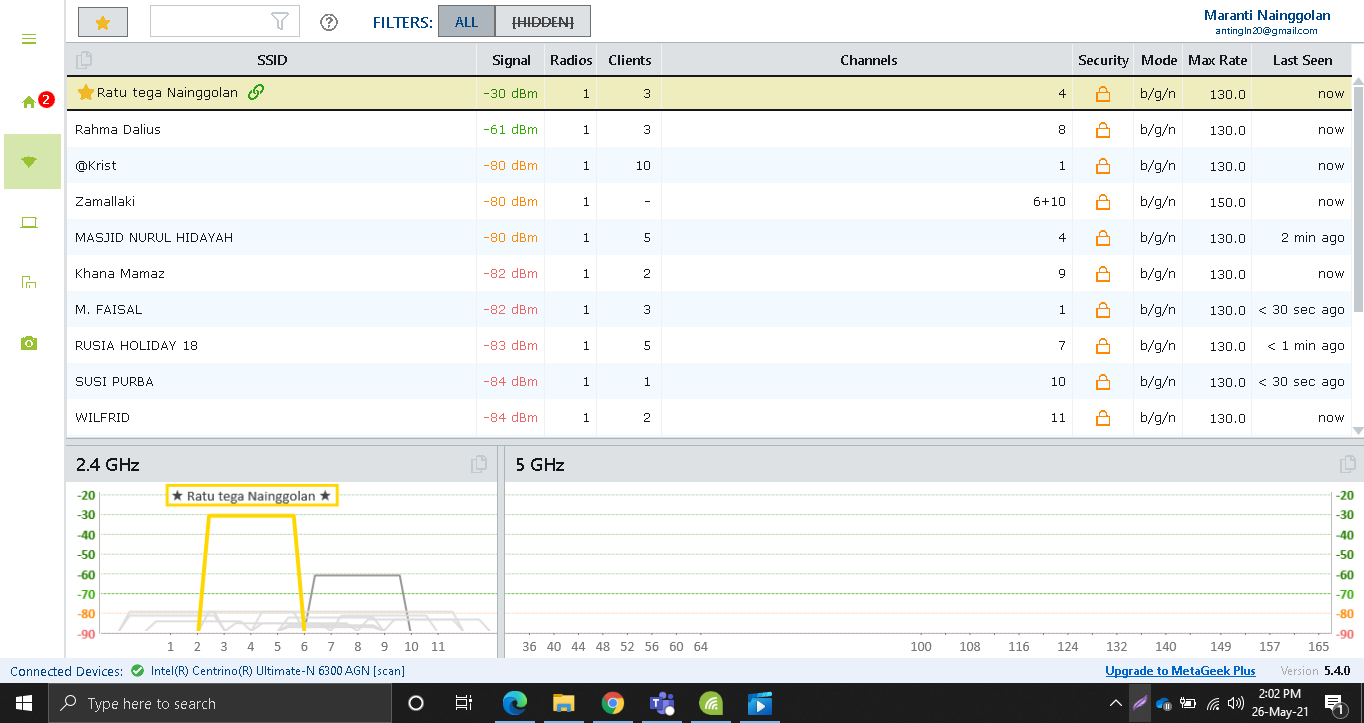
\includegraphics[width=0.4\textwidth]{8.png}
    \caption{Tampilan inSSIDer dalam Rumah}
    \label{tampilan dalam rumah_1}
\end{figure}

\begin{figure}
    \centering
    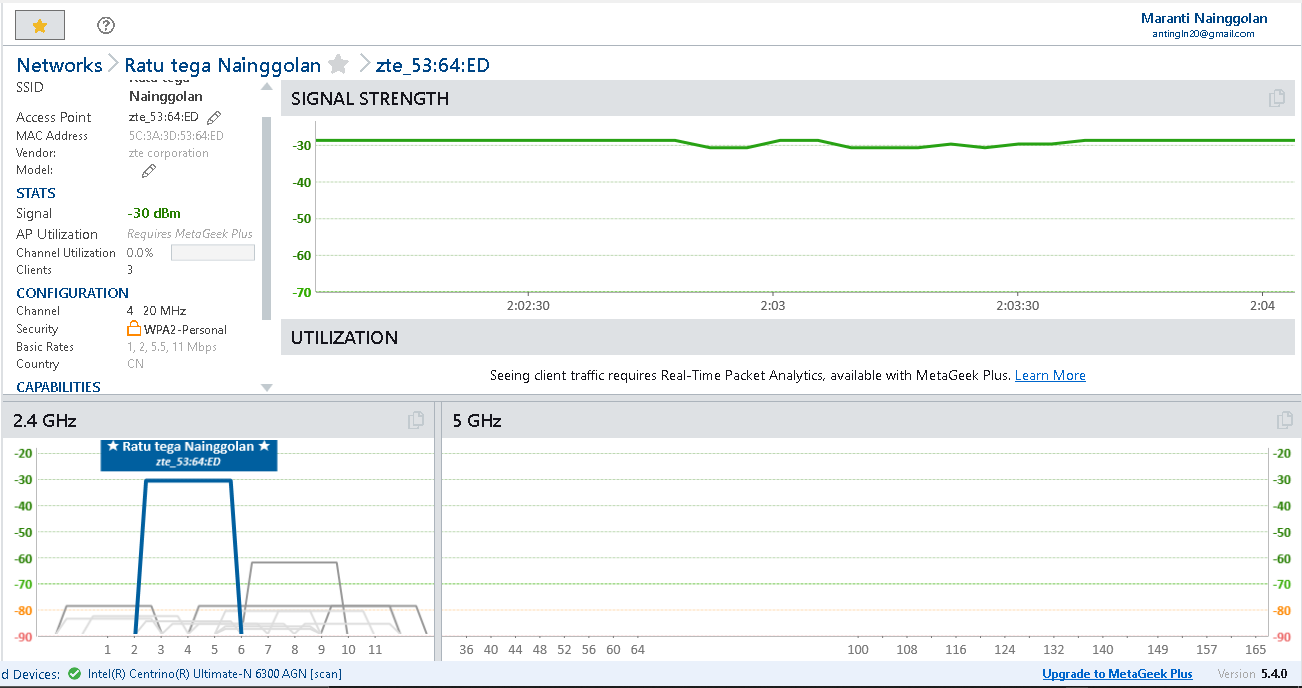
\includegraphics[width=0.4\textwidth]{9.png}
    \caption{Tampilan inSSIDer dalam rumah}
    \label{tampilan dalam rumah_2}
\end{figure}

\vspace{4 cm}

    \item Pengambilan Data dengan Jarak 15 M dari Rumah

    \begin{figure}
        \centering
        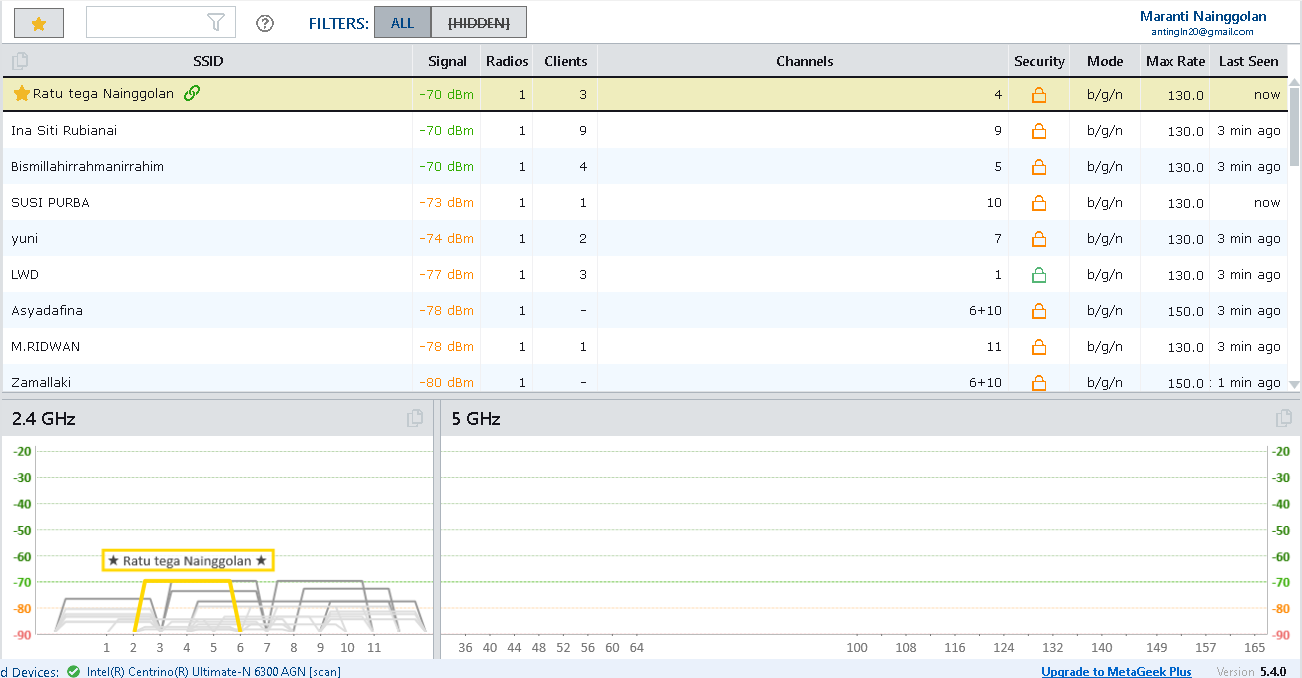
\includegraphics[width=0.4\textwidth]{10.png}
        \caption{Tampilan inSSDer dengan jarak 15 M dari Rumah}
    \end{figure}

    \begin{figure}
        \centering
        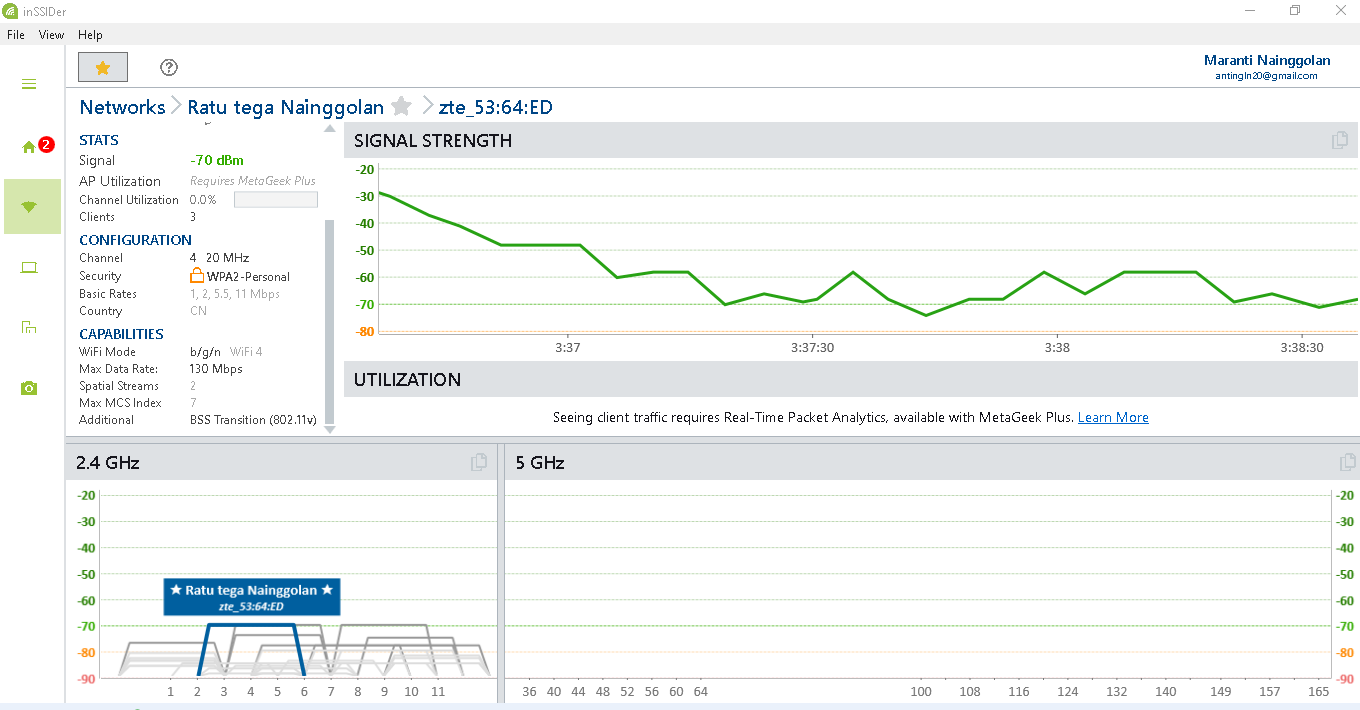
\includegraphics[width=0.4\textwidth]{11.png}
        \caption{Tampilan inSSIDer dengan jarak 15 M dari rumah}
    \end{figure}

\vspace{0.2cm}

Pada gambar diatas terlihat bahwa sinyal wireless dengan
SSID ‘Ratu Tega Nainggolan’ memiliki RSSI (Received
Signal Strength Indicator) yakni -70 dBm. Berada
pada kanal 1 dan bekerja pada frekuensi 2,4 GHz. Menggunakan
model WPA-2 personal security dan memiliki
channel 4
\vspace{0.2cm}  

    \item Pengambilan Data dengan Adanya Penghalang / Pembatas (Dinding)

    \begin{figure}
        \centering
        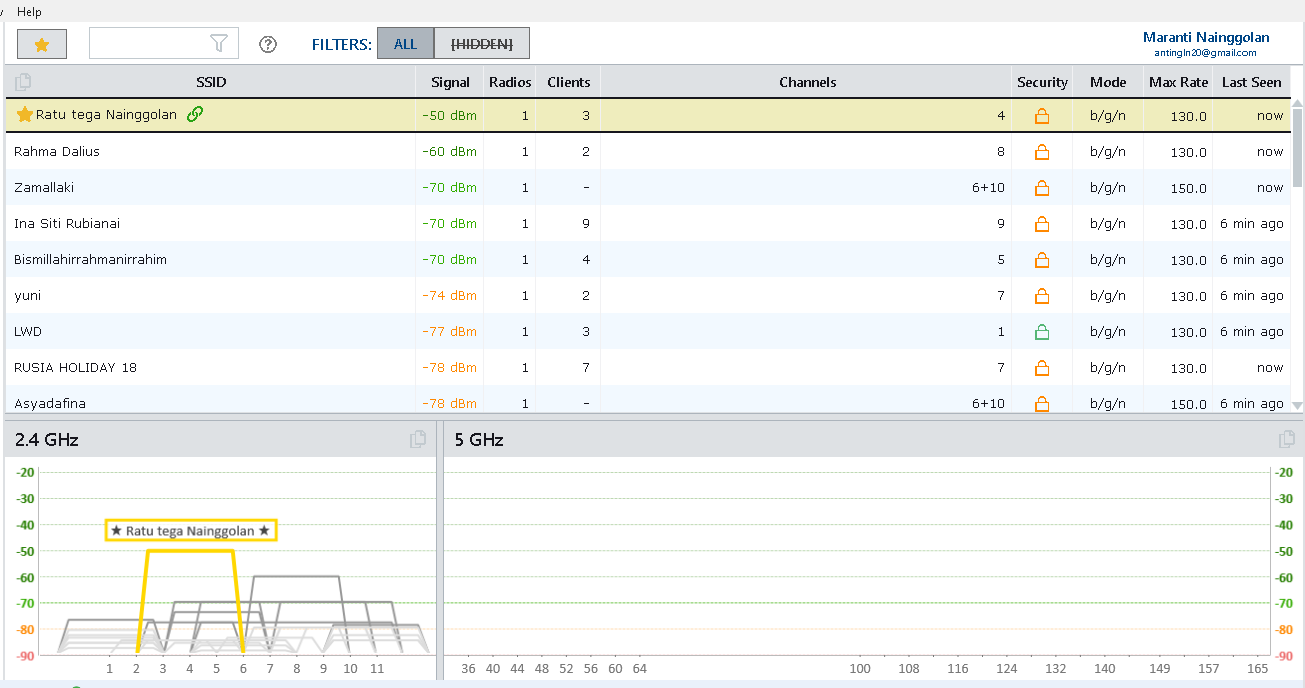
\includegraphics[width=0.4\textwidth]{12.png}
        \caption{Tampilan inSSDer dengan Adanya Pembatas}
        \label{Tampilan dengan Pembatas_1}
    \end{figure}

    \begin{figure}
        \centering
        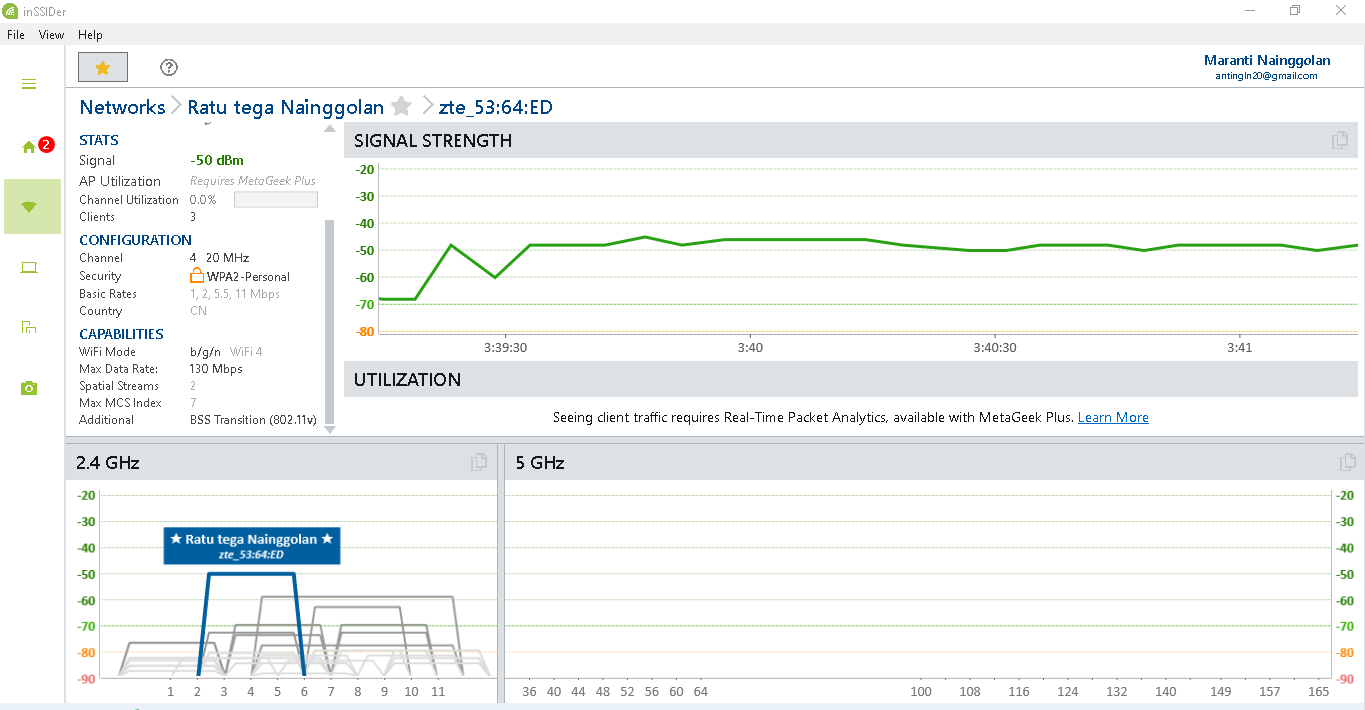
\includegraphics[width=0.4\textwidth]{13.png}
        \caption{Tampilan inSSIDer dengan Adanya pembatas}
        \label{Tampilan dengan Pembatas_2}
    \end{figure}

\vspace{0.2cm}

Pada gambar ~\ref{Tampilan dengan Pembatas_1} dan ~\ref{Tampilan dengan Pembatas_2} terlihat bahwa sinyal wireless
dengan SSID ‘Ratu Tega Nainggolan’ memiliki RSSI (Received Signal Strength Indicator) yakni -50 dBm.
Berada pada kanal 1 dan bekerja pada frekuensi 2,4
GHz. Menggunakan model WPA-2 personal security dan
memiliki channel 4.
\vspace{0.2cm}

    \item Pengambilan Data Saat Berjalan / Mengelilingi Daerah
    Sekitar

\vspace{0.2cm}

Dalam pengambilan kekuatan sinyal wifi saat berjalan,
tentu kekuatan sinyal nya selalu berubah ubah, itu
dikarenan jarak antara pusat wifi dan tempat pengambilan
data, semakin jauh jarak yg ditelusuri maka kekuatan
siyalnya akan terus melemah, begitupun sebaliknya.
\end{itemize}

\vspace{0.2cm}
Dari semua gambar diatas dapat dilihat semua AP menggunakan
atau bekerja di frekuensi 2.4 GHz. Frekuensi
ini memang sering digunakan karena merupakan masuk
dalam standard wireless 802.11b dan 802.11g.Sedangkan
Pada data frekuensi 5 GHz tidak ada AP yang
menggunakannya Terlihat pada panel 5GHz capture
tidak ada SSID yang masuk kategori tersebut.Frekuensi
5GHz ini biasanya digunakan pada 802.11a yang notabennya
memiliki max rate yang sama dengan 802.11g
namun dengan pita yang lebih lebar.

\subsection{Analisis Kekuatan Sinya Dengan adanya Penghalang}
berikut ini adalah hasil dari pengujian kekuatan sinya jika adanya Penghalang~. \cite{b6}

\begin{equation}
    Rerata RSSI = \frac{Total Jumlah Nilai RSSI}{Jumlah Koordinat receiver}
    \label{rerata_rssi}
\end{equation}

berdasarkan persamaan~\ref{rerata_rssi}

\section{Kesimpulan}
Pengambilan data untuk mengetahui kekuatan sinyal Wi-
Fi dengan menggunakan inSSIDer telah dilakukan dengan
baik. Dari semua gambar diatas dapat dilihat semua AP
menggunakan atau bekerja di frekuensi 2.4 GHz. Frekuensi ini
memang sering digunakan karena masuk dalam standard wireless
802.11b dan 802.11g. Sedangkan Pada data frekuensi 5 GHz tidak ada AP yang menggunakannya Terlihat pada panel
5GHz capture tidak ada SSID yang masuk kategori tersebut.
Frekuensi 5GHz ini biasanya digunakan pada 802.11a yang
notabennya memiliki max rate yang sama dengan 802.11g
namun dengan pita yang lebih lebar.

\begin{thebibliography}{00}
    \bibitem{b1} Pranjal., 2013, Experimental Study of a Wireless Local Area Network, International Journal of Information and Computation Technology, Vol.3 No. 10, pp.1047-1052
    \bibitem{b2} Julia Cynthia Rante, Max Alexander Rura Patras. Analisis Kekuatan Sinyal Vol. 14, No. 1, April 2018: 97-102 ISSN: 1907-0837
    \bibitem{b3} Eka, putra, daniel. 2013. Pengamatan Kuat Sinyal Access Point (AP) Menggunakan inSSIDer
    \bibitem{b4} Kapgate, Y., Vatti, R., Jadhav, S., 2017, WiFi Tools and Signal Strength Analysis, GRD Journals Global Research and Development Journal for Engineering , Vol.2 Issue 10.
    \bibitem{b5} https://www.metageek.com/
    \bibitem{b6} Imansyah2019,Analisis Simulasi Pengaruh Uji Kuat Sinyal Wifi Dari Bahan-Bahan Obstacle,https://scholar.google.co.id/
\end{thebibliography}


\end{document}